\documentclass[multi=page, tikz, border=2mm]{standalone}
\usepackage{../tikz-preamble}

% arara: pdflatex: { draft: yes }
% arara: pdflatex: { synctex: no }
% arara: latexmk:  { clean: partial }
\begin{document}

\begin{page}
	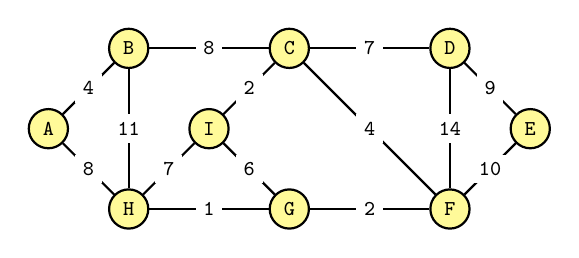
\begin{tikzpicture}[
		scale=0.85,
		transform shape,
		thick,
		font=\ttfamily\bfseries\small
	]
	\tikzset{
		mynode/.style = {circle, draw=black, align=center,fill=yellow!40},
		myedge/.style = {midway, fill=white},
		edgen/.style = {-},
		edger/.style = {-, ultra thick, red},
	}
	\node[mynode] at (0.0,1.2) (a) {A};
	\node[mynode] at (1.2,2.4) (b) {B};
	\node[mynode] at (6.0,2.4) (d) {D};
	\node[mynode] at (3.6,2.4) (c) {C};
	\node[mynode] at (1.2,0.0) (h) {H};
	\node[mynode] at (3.6,0.0) (g) {G};
	\node[mynode] at (6.0,0.0) (f) {F};
	\node[mynode] at (2.4,1.2) (i) {I};
	\node[mynode] at (7.2,1.2) (e) {E};
	%
	\draw[edgen] (a) edge node[myedge] {4} (b);
	\draw[edgen] (b) edge node[myedge] {8} (c);
	\draw[edgen] (c) edge node[myedge] {7} (d);
	\draw[edgen] (d) edge node[myedge] {9} (e);
	%
	\draw[edgen] (a) edge node[myedge] {8} (h);
	\draw[edgen] (h) edge node[myedge] {1} (g);
	\draw[edgen] (g) edge node[myedge] {2} (f);
	\draw[edgen] (f) edge node[myedge] {10} (e);
	%
	\draw[edgen] (h) edge node[myedge] {7} (i);
	\draw[edgen] (i) edge node[myedge] {6} (g);
	\draw[edgen] (i) edge node[myedge] {2} (c);
	%
	\draw[edgen] (b) edge node[myedge] {11} (h);
	\draw[edgen] (d) edge node[myedge] {14} (f);
	\draw[edgen] (c) edge node[myedge] {4} (f);
	\end{tikzpicture}
\end{page}

\begin{page}
    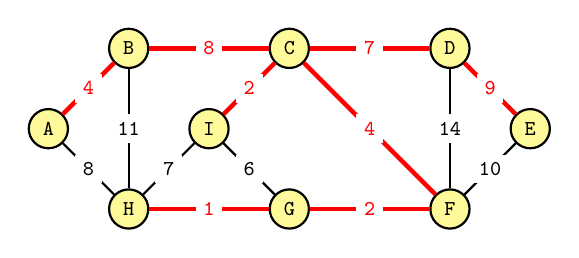
\begin{tikzpicture}[
        scale=0.85,
        transform shape,
        thick,
        font=\ttfamily\bfseries\small
    ]
    \tikzset{
        mynode/.style = {circle, draw=black, align=center,fill=yellow!40},
        myedge/.style = {midway, fill=white},
        edgen/.style = {-},
        edger/.style = {-, ultra thick, red},
    }
    \node[mynode] at (0.0,1.2) (a) {A};
    \node[mynode] at (1.2,2.4) (b) {B};
    \node[mynode] at (6.0,2.4) (d) {D};
    \node[mynode] at (3.6,2.4) (c) {C};
    \node[mynode] at (1.2,0.0) (h) {H};
    \node[mynode] at (3.6,0.0) (g) {G};
    \node[mynode] at (6.0,0.0) (f) {F};
    \node[mynode] at (2.4,1.2) (i) {I};
    \node[mynode] at (7.2,1.2) (e) {E};
    %
    \draw[edger] (a) edge node[myedge] {4} (b);
    \draw[edger] (b) edge node[myedge] {8} (c);
    \draw[edger] (c) edge node[myedge] {7} (d);
    \draw[edger] (d) edge node[myedge] {9} (e);
    %
    \draw[edgen] (a) edge node[myedge] {8} (h);
    \draw[edger] (h) edge node[myedge] {1} (g);
    \draw[edger] (g) edge node[myedge] {2} (f);
    \draw[edgen] (f) edge node[myedge] {10} (e);
    %
    \draw[edgen] (h) edge node[myedge] {7} (i);
    \draw[edgen] (i) edge node[myedge] {6} (g);
    \draw[edger] (i) edge node[myedge] {2} (c);
    %
    \draw[edgen] (b) edge node[myedge] {11} (h);
    \draw[edgen] (d) edge node[myedge] {14} (f);
    \draw[edger] (c) edge node[myedge] {4} (f);
    \end{tikzpicture}
\end{page}

\begin{page}
    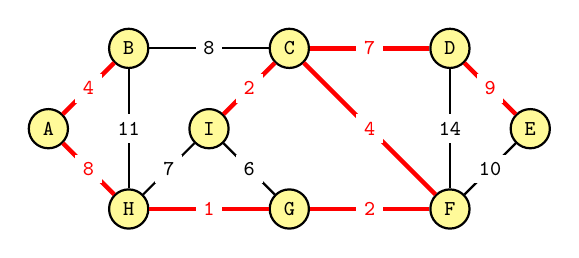
\begin{tikzpicture}[
        scale=0.85,
        transform shape,
        thick,
        font=\ttfamily\bfseries\small
    ]
    \tikzset{
        mynode/.style = {circle, draw=black, align=center,fill=yellow!40},
        myedge/.style = {midway, fill=white},
        edgen/.style = {-},
        edger/.style = {-, ultra thick, red},
    }
    \node[mynode] at (0.0,1.2) (a) {A};
    \node[mynode] at (1.2,2.4) (b) {B};
    \node[mynode] at (6.0,2.4) (d) {D};
    \node[mynode] at (3.6,2.4) (c) {C};
    \node[mynode] at (1.2,0.0) (h) {H};
    \node[mynode] at (3.6,0.0) (g) {G};
    \node[mynode] at (6.0,0.0) (f) {F};
    \node[mynode] at (2.4,1.2) (i) {I};
    \node[mynode] at (7.2,1.2) (e) {E};
    %
    \draw[edger] (a) edge node[myedge] {4} (b);
    \draw[edgen] (b) edge node[myedge] {8} (c);
    \draw[edger] (c) edge node[myedge] {7} (d);
    \draw[edger] (d) edge node[myedge] {9} (e);
    %
    \draw[edger] (a) edge node[myedge] {8} (h);
    \draw[edger] (h) edge node[myedge] {1} (g);
    \draw[edger] (g) edge node[myedge] {2} (f);
    \draw[edgen] (f) edge node[myedge] {10} (e);
    %
    \draw[edgen] (h) edge node[myedge] {7} (i);
    \draw[edgen] (i) edge node[myedge] {6} (g);
    \draw[edger] (i) edge node[myedge] {2} (c);
    %
    \draw[edgen] (b) edge node[myedge] {11} (h);
    \draw[edgen] (d) edge node[myedge] {14} (f);
    \draw[edger] (c) edge node[myedge] {4} (f);
    \end{tikzpicture}
\end{page}

\begin{page}
    \begin{tikzpicture}[
        scale=0.9,
        transform shape,
        thick,
        font=\ttfamily\bfseries\small
    ]
    \tikzset{
        mynodea/.style = {circle, draw=black, align=center,fill=yellow!40},
        mynodeb/.style = {circle, draw=black, align=center,fill=blue!40},
        myedge/.style = {midway, fill=white},
        edgen/.style = {-},
        edger/.style = {-, ultra thick, red},
        edgeb/.style = {-, ultra thick, blue},
    }
        \node[mynodeb] at (0.0,1.2) (a) {A};
        \node[mynodeb] at (1.2,2.4) (b) {B};
        \node[mynodeb] at (6.0,2.4) (d) {D};
        \node[mynodea] at (3.6,2.4) (c) {C};
        \node[mynodea] at (1.2,0.0) (h) {H};
        \node[mynodea] at (3.6,0.0) (g) {G};
        \node[mynodea] at (6.0,0.0) (f) {F};
        \node[mynodea] at (2.4,1.2) (i) {I};
        \node[mynodeb] at (7.2,1.2) (e) {E};
        %
        \draw[edger] (a) edge node[myedge] {4} (b);
        \draw[edgen] (b) edge node[myedge] {8} (c);
        \draw[edgeb] (c) edge node[myedge] {7} (d);
        \draw[edgen] (d) edge node[myedge] {9} (e);
        %
        \draw[edgen] (a) edge node[below] {8} (h);
        \draw[edger] (h) edge node[myedge] {1} (g);
        \draw[edger] (g) edge node[myedge] {2} (f);
        \draw[edgen] (f) edge node[below] {10} (e);
        %
        \draw[edgen] (h) edge node[myedge] {7} (i);
        \draw[edgen] (i) edge node[myedge] {6} (g);
        \draw[edger] (i) edge node[myedge] {2} (c);
        %
        \draw[edgen] (b) edge node[myedge] {11} (h);
        \draw[edgen] (d) edge node[myedge] {14} (f);
        \draw[edger] (c) edge node[myedge] {4} (f);

        % TAGLIO
        \path[draw, dashed] (0.2,0) .. controls (2.4,4.2) and (4.8,4.2) .. (7.0,0);

        % LEGENDA
        \node[ellipse, draw=black, align=center, fill=yellow!40, minimum width=1.5cm, anchor=west] at (8,3.0) (e) {S};
        \node[ellipse, draw=black, align=center, fill=blue!40, minimum width=1.5cm, anchor=west] at (8,2.0) (e) {V-S};
        \node[font=\sffamily, anchor=west, align=left] at (10.0,2.5) {Taglio};
        \node[font=\sffamily, anchor=west, align=left] at (10.0,1.0) {Insieme $A$};
        \node[font=\sffamily, anchor=west, align=left] at (10.0,0.0) {Arco leggero};
        \draw[ultra thick, black, dashed] (8.00,2.5) -- (9.5,2.5);
        \draw[ultra thick, red] (8.00,1.0) -- (9.5,1.0);
        \draw[ultra thick, blue] (8.00,0.0) -- (9.5,0.0);
    \end{tikzpicture}
\end{page}

\begin{page}
	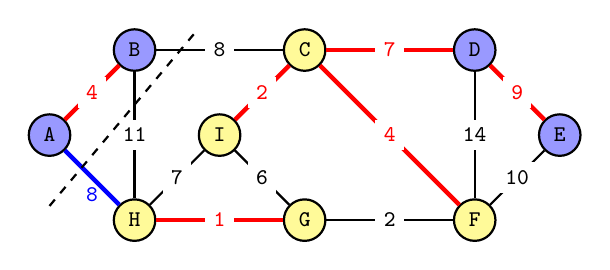
\begin{tikzpicture}[
		scale=0.9,
		transform shape,
		thick,
		font=\ttfamily\bfseries\small
	]
	\tikzset{
		mynodea/.style = {circle, draw=black, align=center,fill=yellow!40},
		mynodeb/.style = {circle, draw=black, align=center,fill=blue!40},
		myedge/.style = {midway, fill=white},
		edgen/.style = {-},
		edger/.style = {-, ultra thick, red},
		edgeb/.style = {-, ultra thick, blue},
	}
		\node[mynodeb] at (0.0,1.2) (a) {A};
		\node[mynodeb] at (1.2,2.4) (b) {B};
		\node[mynodeb] at (6.0,2.4) (d) {D};
		\node[mynodea] at (3.6,2.4) (c) {C};
		\node[mynodea] at (1.2,0.0) (h) {H};
		\node[mynodea] at (3.6,0.0) (g) {G};
		\node[mynodea] at (6.0,0.0) (f) {F};
		\node[mynodea] at (2.4,1.2) (i) {I};
		\node[mynodeb] at (7.2,1.2) (e) {E};
		%
		\draw[edger] (a) edge node[myedge] {4} (b);
		\draw[edgen] (b) edge node[myedge] {8} (c);
		\draw[edger] (c) edge node[myedge] {7} (d);
		\draw[edger] (d) edge node[myedge] {9} (e);
		%
		\draw[edgeb] (a) edge node[below] {8} (h);
		\draw[edger] (h) edge node[myedge] {1} (g);
		\draw[edgen] (g) edge node[myedge] {2} (f);
		\draw[edgen] (f) edge node[myedge] {10} (e);
		%
		\draw[edgen] (h) edge node[myedge] {7} (i);
		\draw[edgen] (i) edge node[myedge] {6} (g);
		\draw[edger] (i) edge node[myedge] {2} (c);
		%
		\draw[edgen] (b) edge node[myedge] {11} (h);
		\draw[edgen] (d) edge node[myedge] {14} (f);
		\draw[edger] (c) edge node[myedge] {4} (f);

		\path[draw,dashed] (0.0,0.2) -- (2.1,2.7);
	\end{tikzpicture}
\end{page}

\begin{page}
    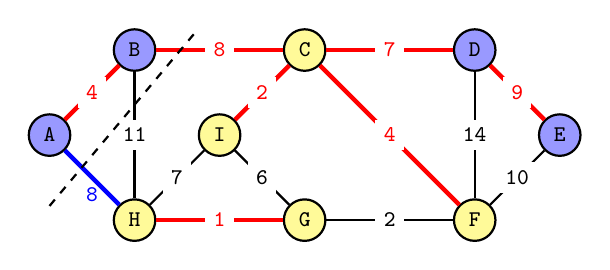
\begin{tikzpicture}[
        scale=0.9,
        transform shape,
        thick,
        font=\ttfamily\bfseries\small
    ]
    \tikzset{
        mynodea/.style = {circle, draw=black, align=center,fill=yellow!40},
        mynodeb/.style = {circle, draw=black, align=center,fill=blue!40},
        myedge/.style = {midway, fill=white},
        edgen/.style = {-},
        edger/.style = {-, ultra thick, red},
        edgeb/.style = {-, ultra thick, blue},
    }
        \node[mynodeb] at (0.0,1.2) (a) {A};
        \node[mynodeb] at (1.2,2.4) (b) {B};
        \node[mynodeb] at (6.0,2.4) (d) {D};
        \node[mynodea] at (3.6,2.4) (c) {C};
        \node[mynodea] at (1.2,0.0) (h) {H};
        \node[mynodea] at (3.6,0.0) (g) {G};
        \node[mynodea] at (6.0,0.0) (f) {F};
        \node[mynodea] at (2.4,1.2) (i) {I};
        \node[mynodeb] at (7.2,1.2) (e) {E};
        %
        \draw[edger] (a) edge node[myedge] {4} (b);
        \draw[edger] (b) edge node[myedge] {8} (c);
        \draw[edger] (c) edge node[myedge] {7} (d);
        \draw[edger] (d) edge node[myedge] {9} (e);
        %
        \draw[edgeb] (a) edge node[below] {8} (h);
        \draw[edger] (h) edge node[myedge] {1} (g);
        \draw[edgen] (g) edge node[myedge] {2} (f);
        \draw[edgen] (f) edge node[myedge] {10} (e);
        %
        \draw[edgen] (h) edge node[myedge] {7} (i);
        \draw[edgen] (i) edge node[myedge] {6} (g);
        \draw[edger] (i) edge node[myedge] {2} (c);
        %
        \draw[edgen] (b) edge node[myedge] {11} (h);
        \draw[edgen] (d) edge node[myedge] {14} (f);
        \draw[edger] (c) edge node[myedge] {4} (f);

        \path[draw,dashed] (0.0,0.2) -- (2.1,2.7);
    \end{tikzpicture}
\end{page}

\begin{page}
    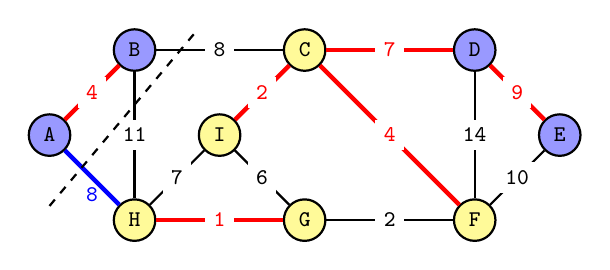
\begin{tikzpicture}[
        scale=0.9,
        transform shape,
        thick,
        font=\ttfamily\bfseries\small
    ]
    \tikzset{
        mynodea/.style = {circle, draw=black, align=center,fill=yellow!40},
        mynodeb/.style = {circle, draw=black, align=center,fill=blue!40},
        myedge/.style = {midway, fill=white},
        edgen/.style = {-},
        edger/.style = {-, ultra thick, red},
        edgeb/.style = {-, ultra thick, blue},
    }
        \node[mynodeb] at (0.0,1.2) (a) {A};
        \node[mynodeb] at (1.2,2.4) (b) {B};
        \node[mynodeb] at (6.0,2.4) (d) {D};
        \node[mynodea] at (3.6,2.4) (c) {C};
        \node[mynodea] at (1.2,0.0) (h) {H};
        \node[mynodea] at (3.6,0.0) (g) {G};
        \node[mynodea] at (6.0,0.0) (f) {F};
        \node[mynodea] at (2.4,1.2) (i) {I};
        \node[mynodeb] at (7.2,1.2) (e) {E};
        %
        \draw[edger] (a) edge node[myedge] {4} (b);
        \draw[edgen] (b) edge node[myedge] {8} (c);
        \draw[edger] (c) edge node[myedge] {7} (d);
        \draw[edger] (d) edge node[myedge] {9} (e);
        %
        \draw[edgeb] (a) edge node[below] {8} (h);
        \draw[edger] (h) edge node[myedge] {1} (g);
        \draw[edgen] (g) edge node[myedge] {2} (f);
        \draw[edgen] (f) edge node[myedge] {10} (e);
        %
        \draw[edgen] (h) edge node[myedge] {7} (i);
        \draw[edgen] (i) edge node[myedge] {6} (g);
        \draw[edger] (i) edge node[myedge] {2} (c);
        %
        \draw[edgen] (b) edge node[myedge] {11} (h);
        \draw[edgen] (d) edge node[myedge] {14} (f);
        \draw[edger] (c) edge node[myedge] {4} (f);

        \path[draw,dashed] (0.0,0.2) -- (2.1,2.7);
    \end{tikzpicture}
\end{page}

\begin{page}
    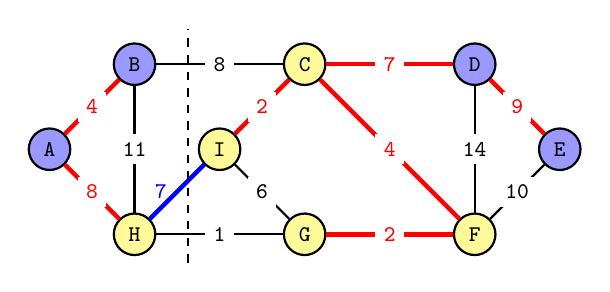
\begin{tikzpicture}[
        scale=0.9,
        transform shape,
        thick,
        font=\ttfamily\bfseries\small
    ]
    \tikzset{
        mynodea/.style = {circle, draw=black, align=center,fill=yellow!40},
        mynodeb/.style = {circle, draw=black, align=center,fill=blue!40},
        myedge/.style = {midway, fill=white},
        edgen/.style = {-},
        edger/.style = {-, ultra thick, red},
        edgeb/.style = {-, ultra thick, blue},
    }
        \node[mynodeb] at (0.0,1.2) (a) {A};
        \node[mynodeb] at (1.2,2.4) (b) {B};
        \node[mynodeb] at (6.0,2.4) (d) {D};
        \node[mynodea] at (3.6,2.4) (c) {C};
        \node[mynodea] at (1.2,0.0) (h) {H};
        \node[mynodea] at (3.6,0.0) (g) {G};
        \node[mynodea] at (6.0,0.0) (f) {F};
        \node[mynodea] at (2.4,1.2) (i) {I};
        \node[mynodeb] at (7.2,1.2) (e) {E};
        %
        \draw[edger] (a) edge node[myedge] {4} (b);
        \draw[edgen] (b) edge node[myedge] {8} (c);
        \draw[edger] (c) edge node[myedge] {7} (d);
        \draw[edger] (d) edge node[myedge] {9} (e);
        %
        \draw[edger] (a) edge node[myedge] {8} (h);
        \draw[edgen] (h) edge node[myedge] {1} (g);
        \draw[edger] (g) edge node[myedge] {2} (f);
        \draw[edgen] (f) edge node[myedge] {10} (e);
        %
        \draw[edgeb] (h) edge node[left] {7} (i);
        \draw[edgen] (i) edge node[myedge] {6} (g);
        \draw[edger] (i) edge node[myedge] {2} (c);
        %
        \draw[edgen] (b) edge node[myedge] {11} (h);
        \draw[edgen] (d) edge node[myedge] {14} (f);
        \draw[edger] (c) edge node[myedge] {4} (f);

        \path[draw,dashed] (1.95,-0.4) -- (1.95, 2.9);
    \end{tikzpicture}
\end{page}

\end{document}